\documentclass[	11pt, ]{fphw}

\usepackage[utf8]{inputenc} 
\usepackage[T1]{fontenc}
\usepackage{mathpazo}\usepackage{graphicx} 
\usepackage{booktabs} 
\usepackage{listings} 
\usepackage{amsmath}
\usepackage{eso-pic}
\usepackage{array}
\usepackage{float}
\usepackage{graphicx}
\usepackage{bbm}
\usepackage{transparent}
\usepackage{indentfirst}
\usepackage{amsthm}
\usepackage{amsmath,amssymb}
\usepackage{subfigure}
\usepackage{tabu}
\usepackage{enumitem}
\usepackage{caption,tabularx,booktabs}
\usepackage{enumerate} 
\usepackage[english]{varioref}

\renewcommand{\thesection}{\Roman{section}}
\usepackage{titlesec}
\titleformat{\section}
{\normalfont\Large\bfseries}{Exercise~\thesection}{1em}{}
\makeatletter
\renewcommand{\@seccntformat}[1]{%
  \csname the#1\endcsname
  \csname suffix@#1\endcsname % this does nothing unless \suffix@... is defined
  \quad
}
% the subsection number is just a letter
\renewcommand{\thesubsection}{\alph{subsection}}
% but references will also have “section.subsection.” in front of the letter
\renewcommand{\p@subsection}{\thesubsection.}
% define \suffix@subsection
\newcommand{\suffix@subsection}{)}
\makeatother

\title{Assignment \#6} %
\author{Anita Mezzetti} 
\institute{École polytechnique fédérale de Lausanne} 
\class{Global Business Environment} 
\professor{Luisa Lambertini} 

%--------------------------------------------------------------------
\begin{document}
\maketitle

\section{}
\subsection{}
False. 
\par The rise in the risk premium of Home bond would reduce the
demand of Home currency, that affects the exchange rate, causing a
depreciation of the Home currency. 
The interest rate parity condition explains these effects. We assume that interest rate is equal to $r_{f }+ \rho $, where $\rho$ is a measure of the risk associated to the asset and $r_{f }$ is the risk free rate. $r_{f }$ is controlled by the IPC. Applying the IPC we obtain
\[R = R^{*} + \frac{E^{e}}{E} - 1 + \rho-\rho^{*}.\]
An increase in the home $\rho$ causes an increase in E, that is a depreciation
of the exchange rate. Since we do not know if the downgrade
is permanent we cannot deduce anything about the expected exchange rate.

\subsection{}
False. 
\par Britain would like to decrease the inflation rate. To do it the Bank of England should apply a permanent decrease in the money supply and increase its policy rate to influence prices in the long run.





\section{}
\subsection{}

The SBN conducts the country’s monetary policy as an independent central bank. It is obliged by the Constitution and by statute to act in accordance with the interests of the country as a whole. Its primary goal is to ensure price stability. A stable system is understood to be a system whose individual components fulfil their individual functions and are resilient to potential shocks. It is an important prerequisite for economic development.
In general, a stabilisation fund is a mechanism set up by a government or central bank to protect the domestic economy from large floods of revenue. A primary motivation is maintaining a steady level of government revenue in the face of major commodity price fluctuations as well as the avoidance of inflation and associated atrophy of other domestic sectors. 
In particular, SBN established a stabilisation fund to maintain price stability. This fund is a special purpose vehicle to which the illiquid assets of UBS were transferred. On 7 November 2013, UBS signed a purchase agreement to acquire the StabFund from the Swiss National Bank (SNB). UBS sold the assets to a SPV
owned by Swiss National Bank. The purchase price amounts will be transferred to the SNB parent company and will have a favourable impact on the 2013 annual result. Swiss National Bank took these measures to stabilise UBS and strengthen Swiss financial system. 
These measures were necessary because UBS’s situation in October 2008 was critical: there were an high exposure to illiquid securities loans and loans in the US and Europe, huge losses suffered due to fall in prices and high level of uncertainty regarding valuation of such positions.Consequently, in UBS outflows of client funds increases sharply and liquidity situation deteriorates. Situation at UBS poses a risk to financial stability in Switzerland and globally.
Thanks to this nontraditional measure, UBS and consequently Swiss financial system stabilised the reduction in balance sheet risks and liquidity injection.In fact the default of this large bank group would have tremendous consequences for the Swiss economy.
At the end the StabFund successfully wound up sooner than expected, without financial loss for the SNB. No troubled assets returned to UBS. This was an unconventional monetary policy because SNB liquidity assistance is only provided in exceptional cases.\\
Concerning the easing, Quantitative easing is a monetary policy whereby a central bank buys predetermined amounts of government bonds or other financial assets in order to inject liquidity directly into the economy. Central banks purchase government securities or other securities from the market in order to increase the money supply and encourage lending and investment. Although Credit easing is a strategy whereby central banks use to ease credit conditions in the economy by buying private sector assets. The goal is to boost liquidity in a troubled market so that the flow of credit and lending increases. Credit easing does not target the level of reserves. It focuses on expanding the asset side of the balance sheet, while quantitative easing is concentrated on the liabilities side. So, we can consider the stabilization fund of SBN a credit easing. 


\subsection{} 
A permanent adoption of a tariff change generates a permanent reduction for the world demand of American goods (domestic country). American products
are more expensive for Europe. Any decrease in relative world demand for U.S. products
causes a deficit of the demand for them at the previous real exchange
rate. \\
We need to reestablish the equilibrium: the relative prices of tradable goods produced in the US will decrease relative to the prices of goods made in Europe. 
Therefore Q, i.e. relative price of Europe’s reference expenditure basket in terms of the United States, will increase and, since it is a permanent change, it implies a long-run
real depreciation of the dollar against the euro. Since we do not any
changes in the long run money supply/demand, we do not have any
variation in the actual prices in the US. Therefore the change in Q will cause a change a long-run exchange rate of the dollar against the euro. 
\[ Q=E^{lr}*\frac{P}{P^{*}}\]
\[ E^{lr}=Q*\frac{P^{*}}{P}= Q*\frac{M*L^{*}}{ M^{*}*L}\]

This long-run nominal depreciation will be reflected in the short run: there is a depreciation of the expected exchange rate, i.e. a rise in E. The next relationship shows the fact that there is a depreciation in the exchange rate, considering that we do not have any changes for the interest rate:
\[R=R^{*}+\frac{E^{e}}{E}-1.\]

\newpage
\subsection{}
\begin{figure}[h!] 
\centering 
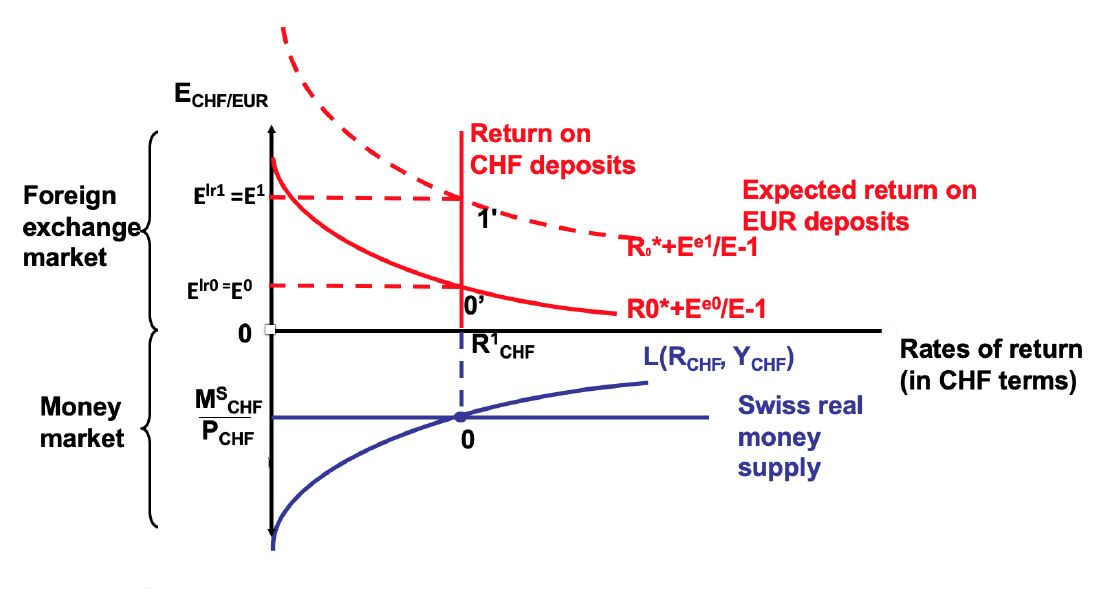
\includegraphics[scale=0.65]{6.JPG} 
\caption{Question 2.c} 
\label{5k}
\end{figure}





\end{document}